\documentclass[11pt]{article}

\usepackage[T1]{fontenc}
\usepackage[utf8]{inputenc}
\usepackage[english]{babel}
\usepackage[a4paper,margin=1in]{geometry}
\usepackage{microtype}
\usepackage{xcolor}
\usepackage{amsmath,amssymb,amsthm}
\usepackage{mathtools}
\usepackage{booktabs,tabularx}
\usepackage{enumitem}
\usepackage{needspace}
\usepackage{flafter}
\usepackage[section]{placeins}
\usepackage{tikz}
\usetikzlibrary{arrows.meta,positioning}
\usepackage{listings}
\usepackage{hyperref}
\usepackage[nameinlink,noabbrev]{cleveref}

\hypersetup{
  colorlinks=true,
  linkcolor=blue!45!black,
  citecolor=green!40!black,
  urlcolor=blue!55!black,
  pdftitle={Compositional Local Branching Analysis for MaxSAT},
  pdfauthor={Anonymous author(s)},
  pdfkeywords={MaxSAT, exact algorithms, automated branching analysis, certificates}
}
\emergencystretch=3em
\widowpenalty=1000
\clubpenalty=1000
\lstset{basicstyle=\small\ttfamily,columns=fullflexible,
  keepspaces=true,frame=single,framerule=0.3pt,
  aboveskip=0.7em,belowskip=0.7em}

\newcommand{\MaxSAT}{\textnormal{\textsc{MaxSAT}}}
\newcommand{\OhStar}{O^*}
\newcommand{\OPT}{\operatorname{OPT}}
\newcommand{\anytail}{\mathord{?}}
\newcommand{\plustail}{\mathord{?}^{+}}
\newcommand{\tail}[1]{\mathord{?}_{#1}}
\newcommand{\ntail}[1]{\mathord{?}^{+}_{#1}}

\newtheorem{theorem}{Theorem}
\newtheorem{lemma}[theorem]{Lemma}
\theoremstyle{definition}
\newtheorem{example}{Example}
\theoremstyle{remark}
\newtheorem{remark}[theorem]{Remark}

% SUBMISSION: Retain anonymity or add affiliations as required by the venue.
\title{Compositional Local Branching Analysis for \MaxSAT{}}
\author{}
\date{}

\begin{document}
\maketitle

\begin{abstract}
Local branching analyses often combine several assignments, reductions, and
further branches before achieving the desired measure decrease. We develop
an automated framework for constructing such analyses for unweighted
\MaxSAT{}. Starting from a partially specified clause neighborhood, the
framework distinguishes possible configurations and searches for sequences of
transformations that preserve an optimal solution and meet a target
running-time bound. It combines local assignment choices with further
reductions and branching on the resulting formulas.
A separate checker validates case coverage, local optimum identities, and
branching inequalities. We apply the framework to the $(3,2)$-literal
bottleneck of the algorithm of~\cite{Xiao2022}. The completed analysis reaches
the target branching base $1.2872$ using branching lemmas from that algorithm, supporting a replacement
of its limiting $(6,6,5,5)$ case. The method combines established ideas in
automated branching into a search for compositional local strategies, with
the case study checked relative to explicitly recorded mathematical
dependencies.
\end{abstract}

\section{Introduction}
\label{sec:introduction}

A local branching analysis describes how a small configuration in an instance
can be replaced by simpler recursive alternatives. To establish a running-time
bound, the alternatives must preserve an optimal solution and decrease the
chosen measure sufficiently. A useful strategy may require several rounds of
branching and reduction, with the choice of later operations depending on the
residual instance. Constructing these strategies and covering all possible
local configurations can require an extensive case analysis.

We study the automation of this task for unweighted \MaxSAT{}, using the
number of clauses as the measure. The input is a partially specified clause
neighborhood together with structural restrictions and a target branching
base. The output is a family of local strategies covering that neighborhood.
Unknown clause tails represent the undisplayed part of the instance, so a
strategy must work for every completion allowed by the restrictions.

Our framework represents groups of local assignments by variable
substitutions. A group can fix some variables and leave others free or
identify them up to sign. Each substitution produces a residual CNF, on which
the search can apply reductions and further branching. The cost of a group
therefore includes its selected continuation. At a fixed target $q$, these
costs are additive, allowing the generator to choose a minimum-weight cover
of the assignments that remain after dominance elimination.

Structural refinement and strategy search serve different roles. Refinement
reveals which local configuration the instance has; a strategy describes how
to solve an instance with that configuration. An analysis script chooses the
refinements and search budgets, while the program searches for strategies
within those choices. A separate checker validates the resulting case analysis
without repeating the optimization search.

Our main application is Step~5.4 of the exact \MaxSAT{} algorithm
of~\cite{Xiao2022}, which we call the \emph{baseline algorithm}.
A branching vector records the guaranteed clause decreases in the recursive
alternatives. The baseline vector $(6,6,5,5)$ limits that algorithm to
$\OhStar(1.2886^m)$ time, where $m$ is the number of clauses and $\OhStar$
suppresses polynomial factors. Our generated analysis reaches the target
$q=1.2872$ using branching lemmas from the same source. The remaining cases
and the terminal algorithm are retained. This is a completed application of
the local method, whose search interface is not specific to Step~5.4.

\paragraph{Contributions.}
We develop a compositional local strategy search combining substitution-based
groups, recursive residual analysis, and selection by continuation costs.
We give a common semantic check for the generated transformations and a
certificate checker for their composition and structural coverage. Finally,
we provide a complete analysis of the selected \MaxSAT{} family at
$q=1.2872$, with its imported mathematical dependencies recorded explicitly.

\subsection{Related work and scope}
\label{sec:related}

Automated branching analysis predates this work. Fedin and
Kulikov~\cite{FedinKulikov2004} generated upper-bound proofs from supplied
simplification rules, including experiments for \MaxSAT{}.
Kulikov~\cite{Kulikov2005} studied automatic discovery of simplification
rules. Skjernaa~\cite[Chapter~8]{Skjernaa2004} used partially specified
formula patterns, structural refinements, reductions, and branching on both
variable values and equality or inequality of pairs of variables. His search
also considers depth-two strategies, with further branching in one or both
children. Thus neither structural case generation nor multistep branching is
new in itself.

Weighted covering is also an established formulation. Gao et
al.~\cite{GaoEtAl2024} select branching rules for Maximum Independent Set
through a weighted set-cover problem with costs evaluated at a fixed
branching base. \v{C}erven\'y and Such\'y~\cite{CervenySuchy2023} generate
branching algorithms for $d$-Path Vertex Cover and provide a separate proof
verification procedure in their accompanying implementation.%\footnote{\url{https://github.com/generating-algorithms/generating-dpvc}}
Our focus is
the combination of substitution-generated residual CNFs, recursive searches
on those residuals, and their continuation costs within a covering search.
The checker validates the resulting local transformations through optimum
identities over unknown tail values. We do not claim priority for dominance,
grouping, fixed-target weights, or separate verification individually.

The framework constructs finite local analyses, rather than solving an
arbitrary global analysis automatically. Its completeness depends on the
chosen refinements and search budgets. Restrictions on a template can describe
other local families, including bounded-width families, but a global bound
for another variant requires its own coverage and recursive-algorithm
argument. Proof logging for individual \MaxSAT{} instances, such as certified
preprocessing~\cite{IhalainenEtAl2024}, has a different target from the
family-wide local analyses considered here.

\section{The local analysis problem}
\label{sec:preliminaries}

We use standard unweighted \MaxSAT{} terminology as in~\cite{Xiao2022}.
A formula $F$ is a multiset of clauses: equal clauses are retained with
multiplicity. We assume the normalization described in
\cref{app:normalization}, and write $m=|F|$ and
\[
  \OPT(F)=\max_{\alpha}\operatorname{sat}(F,\alpha),
\]
where $\alpha$ ranges over all assignments and $\operatorname{sat}$ counts
satisfied clauses with multiplicity. We describe transformations of the
optimum directly.
Throughout, $F\uplus G$ denotes multiset union: clause multiplicities add.

A literal $x$ has degree $(i,j)$ if it occurs in $i$ clauses and its complement
$\bar x$ in $j$ clauses. The complementary literal has degree $(j,i)$.
The degree of the underlying variable is $i+j$.
An $(i,1)$-literal is a \emph{singleton} when its unique
negative occurrence is the unit clause $(\bar x)$.

\subsection{Templates, scores, and measure decreases}
\label{sec:local-notation}

A \emph{template} $P$ is a multiset of displayed clauses. It names selected
variables explicitly and uses a \emph{tail} $\anytail$ for the as-yet-undisplayed
part of a clause. A $\plustail$ tail contains at least one literal, whereas a $\anytail$ tail
may be empty. These marks describe clause syntax, not truth values; even a
nonempty tail may evaluate to false. Subscripts distinguish tails, and repeated
identifiers denote the same disjunction. All occurrences of a selected
variable are displayed. Clauses written consecutively form a multiset, so
repeated clauses count separately.
We call these selected variables the \emph{local variables} of the template.
Child templates may retain them or introduce fresh local variables; in either
case their occurrences are confined to the displayed clauses.

A complete formula \emph{matches} $P$ when it can be written as
$F=P[T]\uplus E$. Here $T$ replaces each tail by a disjunction of literals
on unselected variables, and $E$ contains the remaining clauses.
Even when a clause occurs in both parts, its multiplicities add.
No selected variable occurs in $T$ or $E$. Matching also
respects any degree and singleton restrictions stated for the template.
For a Boolean vector $\tau$ indexed by the tails, define the \emph{local
score}
\begin{equation}
 B_P(\tau)=\max_{\alpha}\operatorname{sat}(P,\alpha,\tau),
 \label{eq:local-score}
\end{equation}
where $\alpha$ assigns the selected variables and each tail is treated as a
Boolean input. A clause made true by a tail counts as one satisfied clause.
Different tails can share hidden variables in a complete instance. Checking
all Boolean vectors $\tau$ includes every realizable combination, and may
therefore reject a valid transformation, but cannot accept an invalid one for
this reason.

A correct branching step produces formulas $F_i$ and nonnegative integer
\emph{offsets} $s_i$ such that
\[
  \OPT(F)=\max_i\bigl(s_i+\OPT(F_i)\bigr).
\]
Its \emph{measure decreases} are $d_i=|F|-|F_i|$. These need not equal the
offsets: an empty false clause contributes to $d_i$ but not to $s_i$.
For example, assigning $x=1$ in $(x)(\bar x)$ gives $s=1$ and $d=2$.
The generator represents such steps locally by transforming templates;
\cref{lem:contextual-replacement} connects a checked local identity to the
corresponding full formulas $F_i$.

\subsection{Fixed-target weights and recurrences}
\label{sec:weights}

For a target $q>1$ and a nonempty integer vector $v=(d_1,\ldots,d_r)$,
define its \emph{fixed-target weight}
\begin{equation}
 W_q(v)=\sum_{i=1}^{r}q^{-d_i}.
 \label{eq:weight}
\end{equation}
Repeated entries are counted separately. A vector of positive integer
decreases is \emph{$q$-admissible} when
\begin{equation}
  W_q(v)\le 1.
  \label{eq:target}
\end{equation}
For a positive decrease vector with at least two entries, its
\emph{branching factor} is the unique $\rho>1$ satisfying
$\sum_i\rho^{-d_i}=1$. Thus $W_q(v)\le1$ means that its branching factor
is at most $q$.
For the case study we use $q=1.2872$; acceptance checks this inequality
exactly. A local recursive call with no additional decrease has vector $(0)$
and weight one. Such a call can end a continuation after a positive incoming
decrease; by itself it does not establish a progressing recursive step.


The local search is successful when every terminal structural case has a
correct strategy whose accumulated call decreases are positive and
$q$-admissible. The target is a test on the complete strategy; an intermediate
branch need not meet it on its own. Standard branching recurrence analysis
then gives an $\OhStar(q^m)$ bound when these strategies are embedded in a
covering global algorithm with polynomial work per node
(\cref{lem:recurrence}).

\section{Search for compositional strategies}
\label{sec:automation}
\label{sec:overview}

The generator maintains a frontier of unresolved templates. A script chooses
when to refine this frontier and when to search for strategies. A successful
search records a strategy and removes its template; generation finishes when
the frontier is empty. \Cref{fig:pipeline} gives the control flow. The
following operations describe the search independently of the particular
\MaxSAT{} neighborhood used in \cref{sec:global}.

\begin{figure}[!htbp]
\centering
\begin{minipage}{0.86\linewidth}
\begin{lstlisting}
frontier <- {root template}
for each command in the analysis script:
    if the command selects a refinement:
        replace selected unresolved templates by their children
    if the command starts a strategy search:
        for each selected unresolved template:
            if a strategy is found, record it and remove the template
require frontier empty
assemble the certificate; check coverage, identities, and vectors
\end{lstlisting}
\end{minipage}
\caption{The generation and checking pipeline. Refinements cover structural
cases; a strategy search resolves cases when it finds a suitable branch or
reduction. The script chooses the refinements and search budgets.}
\label{fig:pipeline}
\end{figure}

\subsection{Structural refinement}

A template represents many possible neighborhoods. To distinguish them, the
generator splits an unknown tail into empty and nonempty cases, or exposes a
literal from a nonempty tail. For an exposure, it enumerates the allowed
oriented degrees and all placements of the literal's remaining occurrences,
adding clauses when necessary. All occurrences of the exposed variable become
displayed. These operations reveal structure of the same complete instance;
they do not assign truth values.

The degree list is supplied by the intended application. In the case study it
comes from the preceding steps of the baseline algorithm. Each refinement must
cover every instance matching its parent under these restrictions. The checker
regenerates the children to validate the enumeration; the completeness of the
degree list is a mathematical premise of the application.

\subsection{Assignments, groups, and residual formulas}
\label{sec:group-search}

Strategy search starts by enumerating assignments to the selected variables.
An assignment can be discarded when another is at least as good for every
valuation of the unknown tails. This is dominance among assignment
alternatives, not deletion of subsumed clauses from a \MaxSAT{} instance.
The remaining assignments must be covered by recursive alternatives.

The generator represents an assignment group by a substitution
\begin{equation}
 x_j\longmapsto 0,\ 1,\ u_1,\ \bar u_1,\ldots,u_t,\bar u_t,
 \label{eq:substitution}
\end{equation}
where the $u_i$ are fresh local variables. For example, $(x,y)=(u,0)$
represents $\{(0,0),(1,0)\}$, and $(x,y)=(u,\bar u)$ represents
$\{(0,1),(1,0)\}$. A group is exactly the image of its substitution.
This representation supports constants and signed identifications, but not
arbitrary Boolean constraints between the free variables.

Substitution yields an ordinary residual CNF, together with an objective offset
and an initial clause decrease. The residual search can apply reductions,
branch on another variable, or stop with a call to the global algorithm.
For each candidate branching variable (pivot), it searches both assignment
children up to a requested depth and retains a deeper continuation when useful.
This allows asymmetric strategies and makes
the group's eventual cost depend on the residual structure it preserves.
Clause-decreasing reductions can end in a call; implemented zero-decrease
reductions eliminate a local variable before continuing.

\subsection{Selection by continuation costs}
\label{sec:fixed-target}

For a strategy $S$, let $v(S)$ denote the vector of accumulated clause
decreases at its recursive-call leaves, measured from the root of $S$.
At a fixed target $q$, an incoming decrease $b$ multiplies a continuation's
weight by $q^{-b}$, and recursive alternatives add their weights:
\begin{equation}
 W_q(b+v)=q^{-b}W_q(v),\qquad
 W_q(v\Vert u)=W_q(v)+W_q(u).
 \label{eq:weight-composition}
\end{equation}
Here $b+v$ adds $b$ to every vector entry, and $\Vert$ concatenates vectors.
For each group, the generator can therefore retain its minimum-weight
available continuation independently of the choices for other groups.
\Cref{lem:weight-selection} formalizes this elementary separability property.
It concerns the supplied candidates, not completeness of the residual search.

Let $A$ be the undominated assignments and $G$ an available substitution
image. If $b_G$ is its initial decrease and $S_G$ its retained continuation,
assign it cost $c_q(G)=q^{-b_G}W_q(v(S_G))$. The generator solves
\begin{equation}
 \min_{\mathcal G}\sum_{G\in\mathcal G}c_q(G)
 \quad\text{subject to}\quad A\subseteq\bigcup_{G\in\mathcal G}G.
 \label{eq:group-cover}
\end{equation}
Groups may overlap and include dominated assignments. Every selected group
contributes its full cost, and its complete substitution image is retained.
The cover search is exhaustive over the supplied candidates, with exponential
worst-case cost. Its result is also compared with ordinary one-level variable
branching.

Standalone branching factors do not give the same ordering of continuations.
For example, $(1,8)$ has smaller branching factor than $(2,5)$, but at
$q=1.2872$ their weights are approximately $0.909568$ and $0.886532$,
respectively. The latter is better inside any fixed enclosing decomposition
with the same incoming decrease. Comparing at the target avoids discarding
it merely because its standalone factor is larger. Search uses floating-point
weights; certificate acceptance checks the selected strategy with exact
rational arithmetic and requires positive accumulated decreases.

\subsection{A worked local strategy}

\begin{example}[A continuation that meets the target]
\label{ex:group}
The following nine-clause template is extracted from the certificate, with
variables and tails renamed:
\begin{equation}
\begin{split}
 P={}&(x\vee\bar y\vee z\vee\tail{1})(x\vee\tail{2})
       (x\vee\tail{3})\\
    & (\bar x\vee y\vee\tail{4})(\bar x\vee\bar y\vee z\vee\tail{5})\\
    & (y\vee\tail{6})(\bar y\vee\bar z\vee\tail{7})
       (z\vee\tail{8})(\bar z\vee\tail{9}).
\end{split}
\label{eq:example-parent}
\end{equation}
All three local variables have degree five. The strategy uses three groups:
$G_0$ fixes $y=0$ and leaves $x,z$ free; $G_1$ fixes $y=1,z=0$ and leaves
$x$ free; $G_2$ fixes $x=y=z=1$. These groups cover seven of the eight
assignments. The omitted assignment $(x,y,z)=(0,1,1)$ is dominated by
$(1,1,1)$: changing $x$ to one satisfies the second and third clauses,
while the two clauses containing $\bar x$ remain true through $y$ or $z$.
This comparison holds for every valuation of the tails.

The substitutions satisfy three, four, and seven clauses, respectively.
Their residual templates are
\begin{align*}
 H_0={}&(x\vee\tail{2})(x\vee\tail{3})(\bar x\vee\tail{4})
         (\tail{6})(z\vee\tail{8})(\bar z\vee\tail{9}),\\
 H_1={}&(x\vee\tail{1})(x\vee\tail{2})(x\vee\tail{3})
         (\bar x\vee\tail{5})(\tail{8}),\\
 H_2={}&(\tail{7})(\tail{9}).
\end{align*}
Tail-only clauses remain in the residuals: for instance, $(\tail{6})$ in
$H_0$ is not known to be satisfied or empty. Counting all residual clauses
gives the initial decreases $(9-6,9-5,9-2)=(3,4,7)$. For every Boolean tail
vector $\tau$, coverage and dominance give the local optimum identity
\begin{equation}
 B_P(\tau)=\max\{3+B_{H_0}(\tau),\,4+B_{H_1}(\tau),\,7+B_{H_2}(\tau)\}
 \label{eq:example-identity}
\end{equation}

Stopping at all three residuals would fail the target test:
$W_{1.2872}((3,4,7))\approx1.003940>1$.
The residual $H_0$, however, contains the $(1,1)$-variable $z$. For any fixed
tail values, choosing $z$ satisfies one of its two clauses and both whenever
at least one of their tails is true. Thus replacing those clauses by
$(\tail{8}\vee\tail{9})$ gives
\[
 R_0=(x\vee\tail{2})(x\vee\tail{3})(\bar x\vee\tail{4})
     (\tail{6})(\tail{8}\vee\tail{9}),
 \qquad B_{H_0}(\tau)=1+B_{R_0}(\tau).
\]
This resolution has offset and decrease one. Continuing on $H_0$ and
stopping at $H_1,H_2$ therefore yields
\[
 v(S)=(3+1,4,7)=(4,4,7),\qquad
 W_{1.2872}(v(S))\approx0.899323<1.
\]
The extra decrease makes this decomposition meet the target, illustrating
why a group's cost includes its residual continuation. All transitions in
this example are explicit and require no imported lemma. The external
formula remains in each of the three recursive calls.
\end{example}

\begin{figure}[!htbp]
\centering
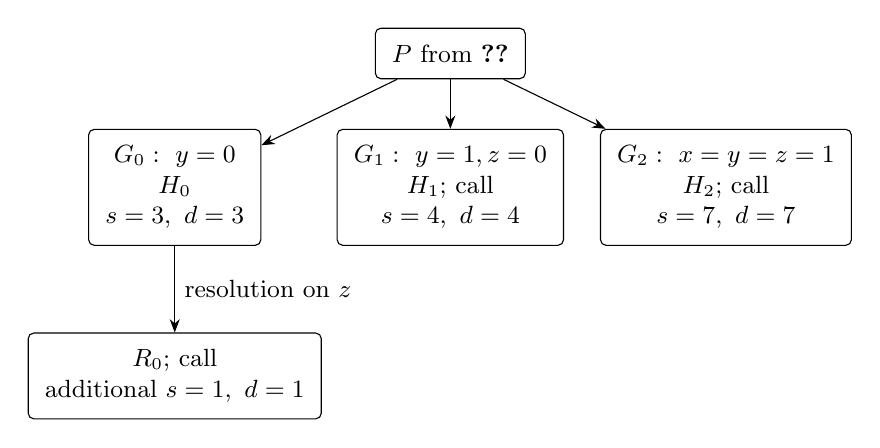
\begin{tikzpicture}[>=Stealth,
 every node/.style={align=center,font=\small},
 case/.style={draw,rounded corners=2pt,inner sep=6pt}]
 \node[case] (p) at (0,0) {$P$ from \cref{eq:example-parent}};
 \node[case] (h0) at (-3.5,-1.7) {$G_0:\ y=0$\\$H_0$\\$s=3,\ d=3$};
 \node[case] (h1) at (0,-1.7) {$G_1:\ y=1,z=0$\\$H_1$; call\\$s=4,\ d=4$};
 \node[case] (h2) at (3.5,-1.7) {$G_2:\ x=y=z=1$\\$H_2$; call\\$s=7,\ d=7$};
 \node[case,below=11mm of h0] (r) {$R_0$; call\\additional $s=1,\ d=1$};
 \draw[->] (p)--(h0);
 \draw[->] (p)--(h1);
 \draw[->] (p)--(h2);
 \draw[->] (h0)--node[right]{resolution on $z$}(r);
\end{tikzpicture}
\caption{The generated decomposition initially has vector $(3,4,7)$.
Resolution in its first residual improves the vector to $(4,4,7)$, meeting
the target $1.2872$. Completions in which hidden literals in the two
$\bar x$-clauses also have degree five satisfy the degree condition of Step~5.4.}
\label{fig:example}
\end{figure}

\section{Correctness and verification}
\label{sec:verification}
\label{sec:implementation-checker}

The checker validates local transformations through their optimum values.
For a proposed decomposition of a parent $P$ into children $H_i$ with offsets
$s_i$, the central test is
\begin{equation}
 B_P(\tau)=\max_i\{s_i+B_{H_i}(\tau)\}
 \quad\text{for every Boolean tail vector }\tau.
 \label{eq:semantic-decomposition}
\end{equation}
Children use only parent tails and local variables, with fresh variables
chosen outside the complete instance. Tail-only clauses that remain are
retained in the recursive formula. For any fixed external assignment, the
identity preserves the best contribution of the local variables; maximizing
over external assignments proves contextual correctness
(\cref{lem:contextual-replacement}). The same test handles reductions,
dominance elimination, and grouped branches.

Composition has two distinct operations. Recursive alternatives contribute
the sum of their shifted weights as in \cref{eq:weight-composition}.
Structural cases describe different possible inputs and contribute their
maximum weight. The checker accumulates decreases along every strategy path,
checks progress at the recursive calls, and checks every structural case.
The local soundness theorem in \cref{thm:local-soundness} gives the formal
guarantee relative to complete structural degree lists and applicable
imported lemmas. The certificate rules and proof are in
\cref{sec:certificate}.

The C++ generator logs refinements and chosen strategies. An assembler connects
them into a certificate and rejects unresolved cases. A separate Python checker
implements template normalization, refinement enumeration, assignment
simplification, local score tables, and exact rational weight arithmetic
independently of the search. Computing a score table for $a$ local variables,
$t$ tails, and representation length $\ell(P)$ takes
$O(2^{a+t}\ell(P))$ time by enumeration. This work concerns the finite offline
analysis. Once its certificate is fixed, local template sizes are constants
with respect to the size of a future input instance.

Imported lemma applications are recorded with their formulas, vectors, and
locations. Their source hypotheses remain mathematical obligations; a
successful checker run does not independently establish those hypotheses.
The implementation is not formally verified. Its acceptance establishes
coverage and the explicit transitions and arithmetic, relative to the stated
structural and imported-result premises. It does not certify that the search
found an optimal strategy.

\section{Application to the \MaxSAT{} bottleneck}
\label{sec:global}

\subsection{The target case and its surrounding algorithm}
\label{sec:bottleneck}

The baseline algorithm of~\cite{Xiao2022}
applies reductions and branching cases in a fixed order. Step~5 handles a
$(3,2)$-literal $x$ with incident clauses
\begin{equation}
 (x\vee C_1)(x\vee C_2)(x\vee C_3)
 (\bar x\vee D_1)(\bar x\vee D_2).
 \label{eq:neighborhood}
\end{equation}
Its Step~5.4 applies when $D_1,D_2$ contain only degree-five variables and
gives the limiting vector $(6,6,5,5)$. The earlier subcases have already
excluded empty incident tails, degree-four literals in $D_1,D_2$, and the
mixed singleton case. The original analysis further distinguishes good
$(3,2)$-literals and their neighboring structures. Our replacement instead
uses the generated family of local strategies.

At $q=1.2872$, the old bottleneck has
$W_q((6,6,5,5))\approx1.00567569>1$. All other baseline recurrences meet
the target. The closest is $(11,3,3)$, with branching factor approximately
$1.287190881$ and weight $0.99997522<1$. Thus this target is determined by
the retained cases. The full table of baseline cases is in
\cref{tab:global-vectors}.

\subsection{The generated family and mathematical dependencies}
\label{sec:configuration}

The analysis starts from
\begin{equation}
 P_0=(x\vee\tail{1})(x\vee\tail{2})(x\vee\tail{3})
     (\bar x\vee\tail{4})(\bar x\vee\tail{5}).
 \label{eq:root}
\end{equation}
All tails are initially arbitrary. This root family deliberately includes
neighboring cases as well as Step~5.4. The allowed exposure classes are
\[
 (3,1)\text{-singleton},\quad (2,2),\quad (3,2),\quad
 (2,3),\quad (4,1)\text{-singleton},
\]
with degrees oriented toward the exposed literal.
The script first exposes $y$ in a clause containing $\bar x$, then $z$ in a
clause containing $\bar x$ but not $y$, interleaving these refinements with
strategy searches. A final tail split and search resolve the remaining cases.


Every instance reaching Step~5.4 belongs to this family. Before Step~5,
the baseline reductions and Steps~1--4 leave only $(2,2)$-variables,
$(3,2)$-variables, and $(3,1)$- or $(4,1)$-singletons
\cite[Section~4.6]{Xiao2022}. A singleton's negative literal occurs only in
its own unit clause, so it cannot be exposed in a clause already containing
another selected variable. The five oriented classes above therefore cover
all possible exposures. Structural refinement reveals occurrences in that
same instance, preserving these restrictions.

The search uses the baseline Lemmas~2--4 and the repeated Lemma~3 argument
from Step~5.5 as available continuation rules. Their source hypotheses,
including reduction-or-branch alternatives, are retained. Step~5.1 is expanded
into an explicitly checked local proof. \Cref{tab:dependencies} lists the
correspondence between the source results and the certificate names;
\cref{sec:strategies} describes their verification boundary.

\subsection{Completed analysis}
\label{sec:artifact}

The generated analysis resolves all cases, and the assembled certificate
passes the separate checker with verdict
\texttt{ACCEPT BOTTLENECK RELATIVE TO IMPORTED LEMMAS}.
\Cref{tab:artifact-summary} summarizes the certificate and the measured costs. These measurements describe
offline construction and checking, not the running time of a \MaxSAT{} solver.

\begin{table}[!htbp]
\centering\small
\begin{tabular}{@{}lr@{}}
\toprule
Property & Value \\
\midrule
Structural refinements & 58 \\
Strategy roots & 7,126 \\
Certificate nodes & 41,825 \\
Maximum depth & 9 \\
Imported applications & 2,632 \\
Generation, wall-clock seconds & 9.31 \\
Assembly, wall-clock seconds & 8.31 \\
Verification, wall-clock seconds & 33.50 \\
\bottomrule
\end{tabular}
\caption{The completed analysis at $q=1.2872$.
Imports are logged mathematical dependencies, not independently proved leaves.}
\label{tab:artifact-summary}
\end{table}

The implementation and analysis artifacts are available in the
\href{https://github.com/kisorimaD/maxsat_prover}{project repository}.
Timings are single runs on an AMD Ryzen~7 5800U with Python~3.10.6 and
NumPy~2.2.6.

\subsection{Consequence for the baseline algorithm}

A fixed certificate gives a finite dispatch procedure for the target family.
A refinement inspects a concrete tail or scans a selected literal's
occurrences and follows a matching child. All templates and strategies have
fixed finite size, so matching and the recorded transformations take
polynomial time and space in the input length. The offline search is not
repeated when solving an input instance.

\begin{theorem}[Global consequence]
\label{thm:conditional-global}
Suppose the completed certificate at $q=1.2872$ satisfies the premises of
\cref{thm:local-soundness}, with the imported results applicable under their
source hypotheses. Replacing Step~5.4 of the baseline algorithm by its
recorded strategies solves \MaxSAT{} in $\OhStar(1.2872^m)$ time and
polynomial space.
\end{theorem}
\begin{proof}
The root covers Step~5.4, and local soundness supplies optimum-preserving
strategies meeting the target. All other branching cases in
\cref{tab:global-vectors} satisfy the same inequality. The terminal
Step~7 uses $\OhStar(1.2576^m)$ time, within the target. Branching weights
bound the sum of terminal costs by $\OhStar(q^m)$, and fixed-certificate
dispatch has polynomial overhead. A depth-first traversal and the
polynomial-space terminal routine preserve polynomial space.
\end{proof}

\section{Conclusion}
\label{sec:conclusion}

Substitution-based assignment groups let local strategy search continue on
residual formulas and account for those continuations during weighted group
selection. Our implementation produces a separately checked analysis of the
\MaxSAT{} bottleneck at $q=1.2872$, relative to recorded imported lemmas.
Applications to further local families require their own structural
restrictions and, for global bounds, a covering recursive algorithm.

\clearpage
\appendix
\section{Normalization conventions}
\label{app:normalization}

Before applying the recursive algorithm, remove duplicate literals within
each clause. Remove tautological clauses with an objective offset of one
each, and empty clauses with offset zero. The initial measure $m$ counts
clauses after this normalization. Equal nonempty clauses are retained as
distinct multiset occurrences. During a transformation, satisfied clauses
contribute to both the objective offset and the measure decrease, whereas
newly empty false clauses contribute only to the measure decrease. A
tail-only clause remains in the recursive instance unless its emptiness or
satisfaction is established.

\section{Templates and certificate rules}
\label{sec:certificate}

This appendix details the certificate checks summarized in
\cref{sec:verification}: refinements cover the relevant
instances, and strategies preserve their optimum. We use $F$ for a complete
recursive formula and $P$ for its displayed template.

\subsection{Unknown tails and the surrounding formula}

For a strategy transformation, not every tail identifier of the parent need
occur in a child; every identifier that does occur must come from the parent.
The checked score identity justifies any disappearance of local clauses or
tails. Structural refinement has a different role. When a variable is exposed
from a tail, the child's tail describes the remainder after that exposure, and
the displayed fragment may acquire further clauses from $E$. Matching is
always interpreted on the same complete instance, even though its displayed
fragment changes.

The local score $B_P(\tau)$ from \cref{eq:local-score} lets the checker compare
such transformations without constructing a complete formula for each choice
of external clauses.

\subsection{Structural refinements}
\label{sec:refinements}

Refinements distinguish formula structure without making a Boolean assignment.
The two basic operations are shown in \cref{fig:refinement}.

\begin{figure}[!htbp]
\centering
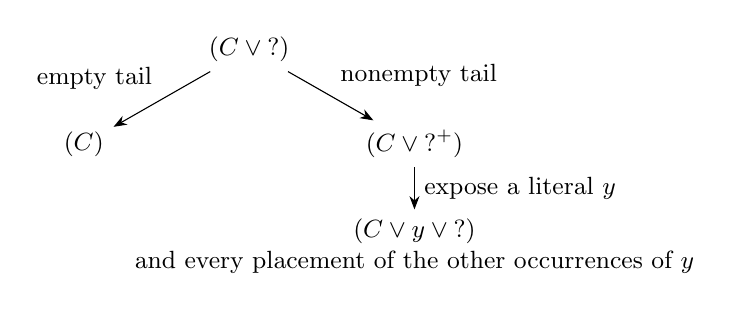
\begin{tikzpicture}[>=Stealth,every node/.style={font=\small,align=center}]
 \node (p) at (0,0) {$(C\vee\anytail)$};
 \node (empty) at (-2.1,-1.2) {$(C)$};
 \node (nonempty) at (2.1,-1.2) {$(C\vee\plustail)$};
 \node (expose) at (2.1,-2.5) {$(C\vee y\vee\anytail)$\\and every placement of the other occurrences of $y$};
 \draw[->] (p)--node[above left]{empty tail}(empty);
 \draw[->] (p)--node[above right]{nonempty tail}(nonempty);
 \draw[->] (nonempty)--node[right]{expose a literal $y$}(expose);
\end{tikzpicture}
\caption{Topological refinement nodes. If $C$ is nonempty, the left child is
an ordinary clause, not an empty clause. After exposing one literal from
$\plustail$, the remaining tail is $\anytail$ and may be empty.}
\label{fig:refinement}
\end{figure}

\paragraph{Tail split.}
Replace a chosen $\anytail$ by the two cases ``empty'' and $\plustail$. These cover every
concrete tail. This is recorded as \texttt{tail\_empty\_or\_nonempty}.

\paragraph{Variable exposure.}
An analysis specifies a finite set of \emph{allowed oriented degrees}
$(i,j)$ for the literal selected from a clause tail. The orientation counts
occurrences of that literal first and its complement second. In our case this
set consists of five classes, listed in \cref{sec:configuration}. Its
completeness follows from the structural assumptions inherited from the baseline
ordered algorithm, not from a bound on clause width.
Choose a literal from a nonempty tail and name it $y$. For each degree in
this set, enumerate all placements of $y$ and $\bar y$ in
existing clause tails, and add clauses for the remaining occurrences.
The selected clause must contain $y$; singleton restrictions fix the unique
negative occurrence to a unit clause. The remaining tail in each affected
clause may be empty. Each concrete occurrence pattern is among these choices,
provided the degree list covers the literals that can be selected.

The format combines a tail split and these exposures in
\texttt{expose\_at\_clause}: an empty child is included for $\anytail$ and omitted
for $\plustail$. Exposure is restricted to templates with distinct, clause-local
single tails. An initial variable declaration constructs the root family;
it is not a refinement of arbitrary formulas.

The coverage requirement can be stated without a separate semantics for
fragments: \emph{every complete instance matching the parent and its
structural restrictions must match at least one child}. Exposing $y$ merely
moves all its occurrences into the displayed fragment of that same instance.
The checker regenerates the child templates, compares them up to renaming,
and rejects missing, extra, or duplicate cases. In format version~2 the
allowed degree list is recorded in the exposure node. Its completeness under
the intended structural restrictions is a mathematical premise, whereas
faithful enumeration of its incidences is checked computationally.

\subsection{Local strategies}
\label{sec:strategies}

The basic certificate operations are refinement, decomposition, recursive
call, and imported lemma application. Refinements may occur within a strategy
as well as above its root. Proof-backed local lemmas and partially expanded
imported lemmas extend these operations as described below.
Decompositions have two forms.

\paragraph{Assignment decomposition.}
The alternatives assign a selected variable $x$ to $0$ and $1$. The checker
simplifies both children and recomputes their offsets and decreases. Suppose
an assignment leaves a displayed fragment $P_i$ and transfers a multiset $R_i$
of tail-only clauses to the surrounding formula. Then
\begin{equation}
 F_i=P_i[T]\uplus E\uplus R_i[T],\qquad
 d_i=|P|-|P_i|-|R_i|.
 \label{eq:transfer}
\end{equation}
Satisfied clauses contribute to $s_i$; empty false clauses contribute only to
$d_i$. The transferred clauses remain part of the recursive instance.
For example, setting $x=0$ in $(x\vee\anytail)(\bar x)$ transfers $(\anytail)$ and gives
$s=d=1$, even though no selected variable remains.

\paragraph{Semantic decomposition.}
The certificate supplies children $H_1,\ldots,H_r$ and offsets $s_i$. The
checker accepts the transformation when
\cref{eq:semantic-decomposition} holds.
Every child uses only parent tails and selected or fresh local variables.
Here the surrounding formula is unchanged, so tail-only clauses that remain
must be included in $H_i$. The decrease is
$d_i=|P|-|H_i|$. A one-child decomposition describes a reduction; its offset
can also be inferred if $B_P-B_{H_1}$ is a constant nonnegative integer.

\Needspace{13\baselineskip}
\begin{lemma}[Replacement inside a formula]
\label{lem:contextual-replacement}
Suppose \cref{eq:semantic-decomposition} holds and the local variables of the
parent and children occur nowhere in the surrounding formula or the concrete
tails. Then replacing $P[T]$ by the alternatives $(H_i[T],s_i)$ preserves the
optimum of $P[T]\uplus E$.
\end{lemma}
\begin{proof}
Fix an assignment $\beta$ to all external variables. It gives tail values
$\tau_\beta$ and satisfies some $e(\beta)$ clauses in $E$. The parent optimum
is
\[
 \max_\beta\bigl(e(\beta)+B_P(\tau_\beta)\bigr)
 =\max_i\left(s_i+
   \max_\beta\bigl(e(\beta)+B_{H_i}(\tau_\beta)\bigr)\right),
\]
using \cref{eq:semantic-decomposition}. The expression on the right is the
best shifted optimum of a child in the same surrounding formula.
\end{proof}

\paragraph{Checked reductions.}
The generator records reductions from \texttt{RR1}--\texttt{RR9} as
one-child semantic decompositions. The checker verifies that the difference
between the parent and child optima is the same nonnegative offset for every
boundary valuation. It computes the decrease from the clause counts.

\paragraph{Recursive call and imported lemma.}
A \texttt{call} ends the local analysis and invokes the global algorithm on
the remaining complete formula. The decrease accumulated along the path is
the decrease of this leaf. An imported lemma application, encoded as
\texttt{assumption}, supplies the vector for the named lemma's branching
case. The checker records its name, formula, vector, and tree path. Its
mathematical justification comes from the cited result and its applicability
to the current instance. Lemmas~2--4 also permit a reduction of at least one
clause, so for a branching vector $v$ the checker uses
\begin{equation}
 \max\{q^{-1},W_q(v)\}.
 \label{eq:imported-lemma-weight}
\end{equation}
For an isolated Lemma~3 application the branching vector contains a decrease
of one, so its weight always exceeds $q^{-1}$. For Lemmas~2 and~4 the
reduction can have the larger weight. The certificate uses the baseline Lemmas~2--4,
together with the repeated Lemma~3 argument
in Step~5.5 of that algorithm. In particular, we use Lemma~3
of~\cite{Xiao2022}, a refinement of Lemma~9 of~\cite{XuEtAl2019}.
These numbers refer to the source results, not to the numbered statements
of this paper. \Cref{tab:dependencies} gives the correspondence to the
certificate names; Step~5.1 is supplied by a checked local proof.

\begin{table}[!htbp]
\centering\small
\begin{tabularx}{\linewidth}{@{}lX@{}}
\toprule
Certificate name & Mathematical dependency \\
\midrule
\texttt{lemma2} & Lemma~2 for an $(i,1)$ literal,
imported there from~\cite{XuEtAl2019}. \\
\texttt{lemma3} & Lemma~3 for a degree-three variable,
refining Lemma~9 of~\cite{XuEtAl2019}. \\
\texttt{lemma4} & Lemma~4 for specified unit occurrences. \\
\texttt{double\_lemma3} & The composition of Lemma~3
used in its Step~5.5,
with the second singleton preserved in the resolution child. \\
\texttt{step5.1} & Step~5.1, the unit-clause case for a
$(3,2)$-literal, supplied by a checked assignment proof. \\
\bottomrule
\end{tabularx}
\caption{Branching dependencies from~\cite{Xiao2022} and their certificate
names. Lemma and step numbers in this table belong to that source.
Imported uses require the source
hypotheses, including any reduction-or-branch alternative and the claimed
decreases in the complete instance. Opaque imported applications are logged;
proof-backed applications are expanded and checked.}
\label{tab:dependencies}
\end{table}

\paragraph{Composing two applications of Lemma~3 from~\cite{Xiao2022}.}
Consider the branching case of that source lemma for a $(2,1)$-singleton $y_1$.
Its resolution child replaces
\[
 (y_1\vee A)(y_1\vee B)(\bar y_1)
 \quad\text{by}\quad (A)(B)
\]
with offset and decrease one. In this case $A$ and $B$ are nonempty; short
clauses that trigger the source reductions are handled before this branching
case. Removing $y_1$ from these two clauses preserves every occurrence of any
other variable, since clause multiplicities are retained. In particular, a
distinct $(2,1)$-singleton $y_2$ retains its two positive occurrences and its
negative unit clause. When the branching case of the same source lemma applies again, the
two nested vectors $(1,8)$ give
\[
 (8,\ 1+8,\ 1+1)=(8,9,2).
\]
This is the composition used in Step~5.5 of the baseline algorithm. If the
second application gives a reduction, the composed vector is covered by
$(8,2)$, whose weight is smaller than that of $(8,9,2)$. A reduction in the
first application gives a single decrease of at least one, so the checker
uses \cref{eq:imported-lemma-weight} with $v=(8,9,2)$.

\paragraph{Step 5.1.}
The generator expands Step~5.1 into an assignment node on the $(3,2)$
variable. The checker reconstructs both residual formulas and their clause
decreases. Only the complete enclosing strategy must meet the target.

\subsection{Composition and soundness}
\label{sec:checker}

A decomposition edge with decrease $d$ followed by a child vector
$(e_1,\ldots,e_t)$ contributes $(d+e_1,\ldots,d+e_t)$ to the enclosing
strategy. Concatenating the vectors of all alternatives gives its leaf
vector. The complete accumulated vector in every structural case must have
positive entries and satisfy \cref{eq:target}; an intermediate reduction
may have decrease zero.
Refinement children are separate structural cases, so their vectors are
not concatenated. At an outer refinement each case is checked separately.
Within a strategy their contribution is bounded by the maximum of the case
weights; an incoming decrease scales this maximum just as it scales a
single continuation.

The identities in \cref{eq:weight-composition} show how weights compose.
Thus recursive alternatives add their shifted weights, whereas structural
cases contribute their worst weight. Both operations preserve an improvement
of any child weight at the fixed target.

\begin{lemma}[Independent continuation selection]
\label{lem:weight-selection}
Fix $q>1$ and a decomposition with incoming decreases $d_g$ for its
alternatives $g=1,\ldots,k$. For each alternative let $\mathcal C_g$ be
a finite nonempty set of available correct continuations, each with positive
accumulated decreases after its incoming edge. Suppose these choices are
independent. Then the minimum weight of the composed strategy is
\begin{equation}
 \min_{(S_g)\in\prod_g\mathcal C_g}
   \sum_g q^{-d_g}W_q(v(S_g))
 =\sum_g q^{-d_g}\min_{S_g\in\mathcal C_g}W_q(v(S_g)).
 \label{eq:independent-selection}
\end{equation}
\end{lemma}
\begin{proof}
By \cref{eq:weight-composition}, the left-hand objective is the weight of
the composed leaf vector. Each coefficient $q^{-d_g}$ is positive, and
each summand depends only on $S_g$. Choosing a minimizing continuation
in every set $\mathcal C_g$ attains the right-hand side; every other
choice has weight at least that value.
\end{proof}
The statement concerns the available continuations at a fixed target.
It does not assert that a bounded search discovers all possible strategies.

\Needspace{17\baselineskip}
\begin{theorem}[Local certificate soundness]
\label{thm:local-soundness}
Let a finite certificate pass the refinement, decomposition, and vector
checks above at target $q$, with positive accumulated call decreases in
every structural case. Suppose its exposure degree lists are complete
under the stated structural restrictions, and each recorded imported lemma
applies with its stated reduction or branching guarantees to every complete
instance at that leaf. Then every such instance
matching the root has an optimum-preserving local strategy whose accumulated
decreases are $q$-admissible.
\end{theorem}
\begin{proof}
Induct over the certificate. A tail split covers its parent, and variable
exposure enumerates every permitted incidence pattern. Thus at least one
refinement child applies to each matching instance. Assignment decomposition
is exhaustive, with the clause accounting in \cref{eq:transfer}. Semantic
decomposition preserves the optimum by \cref{lem:contextual-replacement}.
Calls end a local path, and imported applications use the stated hypothesis.
The maximum in \cref{eq:imported-lemma-weight} bounds both source alternatives.
Edge decreases telescope along each path; larger actual decreases can only
improve \cref{eq:target}. Taking a maximum at an internal refinement bounds
every structural case by \cref{eq:weight-composition}.
The check at each strategy root establishes the
claimed recurrence.
\end{proof}

\section{Retained recurrences}
\label{app:recurrences}

\begin{lemma}[Branching recurrence]
\label{lem:recurrence}
Suppose each recursive step has positive decreases satisfying
\cref{eq:target}, and the work at each node, including any intervening
reductions, is polynomial in the input length. Then the running time is
$\OhStar(q^m)$.
\end{lemma}
\begin{proof}
Induction on $m$ bounds the number of leaves by $q^m$: an internal node has
at most $\sum_i q^{m-d_i}\le q^m$ descendant leaves. Each root-to-leaf path
has at most $m$ recursive edges, since every decrease is positive. The number
of nodes is therefore at most $(m+1)q^m$. Polynomial work per node gives
the claimed bound.
\end{proof}

\begin{table}[!htbp]
\centering\small
\begin{tabularx}{\linewidth}{@{}lXlr@{}}
\toprule
Step & Literal or case type & Branching vector & Base \\
\midrule
1 & Degree at least six & $(6,1)$ & $1.2852$ \\
2 & $(i,1)$ non-singleton, $i\ge3$ & $(3,3)$ & $1.2600$ \\
3 & Degree three & $(8,1)$ & $1.2321$ \\
4 & Unit-clause case & $(5,2)$ & $1.2366$ \\
5.1 & $(3,2)$, unit-clause case & $(4,2)$ & $1.2721$ \\
5.2 & $(3,2)$ & $(11,3,3)$ & $1.2872$ \\
5.3 & $(3,2)$ & $(6,1)$ & $1.2852$ \\
\textbf{5.4} & \textbf{$(3,2)$ bottleneck} & $\mathbf{(6,6,5,5)}$ & $\mathbf{1.2886}$ \\
5.5 & $(3,2)$ & $(11,10,4,3)$ & $1.2801$ \\
6.1 & $(2,2)$ & $(4,2)$ & $1.2721$ \\
6.2 & $(2,2)$ & $(6,1)$ & $1.2852$ \\
6.3 & $(2,2)$ & $(11,3,3)$ & $1.2872$ \\
6.4 & $(2,2)$ & $(18,18,11,11,11,11,4,4)$ & $1.2870$ \\
7 & $(3,1)$- or $(4,1)$-singletons & Set Cover Problem & $1.2576$ \\
\bottomrule
\end{tabularx}
\caption{Baseline cases, adapted from Table~3 of~\cite{Xiao2022}.
Bases reproduce the source's displayed values; for Step~7 the base is
that of the terminal algorithm. We replace the highlighted Step~5.4 by
a family of local strategies checked at $q=1.2872$.}
\label{tab:global-vectors}
\end{table}

\begin{thebibliography}{99}

\bibitem{Xiao2022}
Mingyu Xiao.
\newblock An exact MaxSAT algorithm: Further observations and further
improvements.
\newblock In \emph{Proceedings of the Thirty-First International Joint
Conference on Artificial Intelligence}, pages 1887--1893, 2022.

\bibitem{FedinKulikov2004}
Sergey S. Fedin and Alexander S. Kulikov.
\newblock Automated proofs of upper bounds on the running time of splitting algorithms.
\newblock In \emph{IWPEC}, volume 3162 of LNCS, pages 248--259, 2004.
\newblock \href{https://doi.org/10.1007/978-3-540-28639-4_22}{doi:10.1007/978-3-540-28639-4\_22}.

\bibitem{Kulikov2005}
Alexander S. Kulikov.
\newblock Automated generation of simplification rules for SAT and MAXSAT.
\newblock In \emph{SAT}, volume 3569 of LNCS, pages 430--436, 2005.
\newblock \href{https://doi.org/10.1007/11499107_35}{doi:10.1007/11499107\_35}.

\bibitem{Skjernaa2004}
Bjarke Skjernaa.
\newblock \emph{Exact Algorithms for Variants of Satisfiability and Colouring Problems}.
\newblock PhD thesis, University of Aarhus, BRICS DS-04-5, 2004. Chapter~8.
\newblock \url{https://www.brics.dk/DS/04/5/BRICS-DS-04-5.pdf}.

\bibitem{CervenySuchy2023}
Radovan \v{C}erven\'y and Ond\v{r}ej Such\'y.
\newblock Generating faster algorithms for $d$-Path Vertex Cover.
\newblock In \emph{WG}, pages 157--171, 2023.
\newblock \href{https://doi.org/10.1007/978-3-031-43380-1_12}{doi:10.1007/978-3-031-43380-1\_12}.

\bibitem{GaoEtAl2024}
Xuan-Zhao Gao, Yi-Jia Wang, Pan Zhang, and Jin-Guo Liu.
\newblock Automated discovery of branching rules with optimal complexity for
  the Maximum Independent Set problem.
\newblock arXiv:2412.07685, 2024.
\newblock \url{https://arxiv.org/abs/2412.07685}.

\bibitem{XuEtAl2019}
Chao Xu, Wenjun Li, Yongjie Yang, Jianer Chen, and Jianxin Wang.
\newblock Resolution and domination: An improved exact MaxSAT algorithm.
\newblock In \emph{Proceedings of the Twenty-Eighth International Joint
Conference on Artificial Intelligence}, pages 1191--1197, 2019.

\bibitem{ChenXuWang2017}
Jianer Chen, Chao Xu, and Jianxin Wang.
\newblock Dealing with 4-variables by resolution: An improved MaxSAT algorithm.
\newblock \emph{Theoretical Computer Science}, 670:33--44, 2017.

\bibitem{IhalainenEtAl2024}
Hannes Ihalainen, Andy Oertel, Yong Kiam Tan, Jeremias Berg,
Matti J\"arvisalo, Magnus O. Myreen, and Jakob Nordstr\"om.
\newblock Certified MaxSAT preprocessing.
\newblock In \emph{IJCAR}, volume 14739 of LNCS, pages 396--418, 2024.
\newblock \href{https://doi.org/10.1007/978-3-031-63498-7_24}{doi:10.1007/978-3-031-63498-7\_24}.

\end{thebibliography}
\end{document}
